\subsection{Analyse der Ergebnisse} \label{analyse-subsec}


\begin{table}[H] \centering
\begin{tabular}{|c|c|c|}
\hline
\textbf{F1-Score (\%)} & \textbf{Probanden-abhängig} & \textbf{Probanden-unabhängig} \\ \hline
\textbf{Handgefertigte Merkmale} & 91,49\% & 28,85\% \\ \hline
\textbf{Codebook Approach} & 42,67\% & - \\ \hline
\textbf{Deep Neural Networks} & 47,99\% & 30.91\% \\ \hline
\end{tabular} \vspace{0.2cm} \label{tab-res-1} \caption{Vergleich der Ergebnisse der unterschiedlichen Merkmalsextraktionen.}
\end{table}





Obwohl die handgefertigten Merkmale hier die besten Ergebnisse erzielt haben, wird davon ausgegangen, dass die Performance in Realität deutlich abnehmen könnte.
Der Hauptgrund dafür ist ein sehr Wahrscheinliches Overfitting zu den einzelnen Probanden. 
Unterstüzt wird das durch eine vorläufige qualitative Analyse mithilfe der t-Distributed Stochastic Neighbor Embedding (t-SNE) Methode (siehe Abbildung \ref{fig:overfitting}). 
Oben sieht man die Labels entsprechend den Emotionen und unten entsprechend der Probanden.
Es ist klar zu erkennen, dass die Probanden klarere Klassen bilden und damit die handgefertigten Merkmale nicht Testpersonen-unabhängig klassifizieren. \\


\begin{figure}[H]
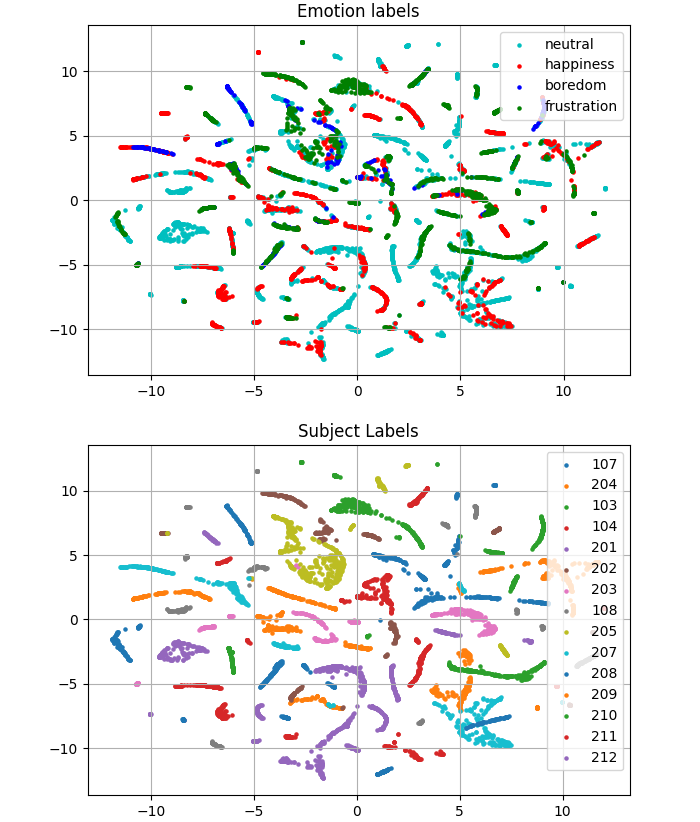
\includegraphics[width=\textwidth]{Images/HCF-tSNE.png} 
\vspace{-0.3cm} \caption{ t-SNE Plots der handgefertigten Merkmale. }
\label{fig:overfitting} \end{figure} \vspace{0.5cm}


Desweiteren wurden an einem Probanden-unabhängigen Datensatz ausgetestet, woraufhin die Performance von 91,49\% auf nur 28,85\% sehr stark sank.
Aus diesen Gründen werden die handgefertigten Merkmale wahrscheinlich mehr von den einzelnen Probanden beeinflußt, als von den unterschiedlichen Emotionen an sich. \\ 





Entgegen unserern Erwartungen liefert der CA sch{\"a}chere Performance als die handgefertigten Merkmale. 
Der Grund hierf{\"u}r ist aber sehr wahrscheinlich der selbe wie bei den  DNNs, und zwar der relativ kleine Datensatz. 
Eine kleine qualitative Analyse der in der Studie verwendeten Daten kann die Gr{\"u}nde f{\"u}r diese Beobachtungen begr{\"u}nden. 
CA-Merkmale (sowohl f{\"u}r weiche als auch f{\"u}r harte Zuweisungen) sind per Definition sehr empfindlich gegen{\"u}ber Variationen der Formen der Originalsignale: Die Codew{\"o}rter werden durch Clustering auf S{\"a}tzen von Segmenten bestimmt, die aus den Originalsignalen extrahiert wurden, und die histogrammbasierten Merkmale selbst basieren auf direkten Vergleichen zwischen den Codew{\"o}rtern und dem Segment der zu klassifizierenden Daten. 
Daher kann jede Quelle von Rauschen oder Unregelm{\"a}{\ss}igkeiten in den Originaldaten die Effektivit{\"a}t der CA-Funktionen stark beeintr{\"a}chtigen. 
Ein Blick auf die in unserer Studie verwendeten Signale ergab zwei Hauptprobleme: falsche Datenwerte, die durch Hardwareprobleme bei einigen Sensoren verursacht wurden (wie in Abbildung \ref{fig:bad_signals}), und das Vorhandensein von Rauschen, das Unregelm{\"a}{\ss}igkeiten in den Signalformen verursacht (siehe Abbildung \ref{fig:zoom}). 
Da der CA schon bei dem Probanden-abhängigen Datensatz keine vielversprechende Ergebnisse aufweiste, wurde darauf verzichtet den CA bei dem Probanden-unabhängigen Datensatz zu testen.
Aus diesem Grund ist in Tabelle \ref{tab-res-1} an der entsprechenden Stelle nur ein ``-'' eingefügt worden.
M{\"o}gliche L{\"o}sungen zur Behebung dieses Problems k{\"o}nnten sein, zus{\"a}tzliche Vorverarbeitungstechniken zur Rauschunterdr{\"u}ckung einzusetzen, wie z.B. Tiefpassfilterung. \\


\begin{figure}[H]
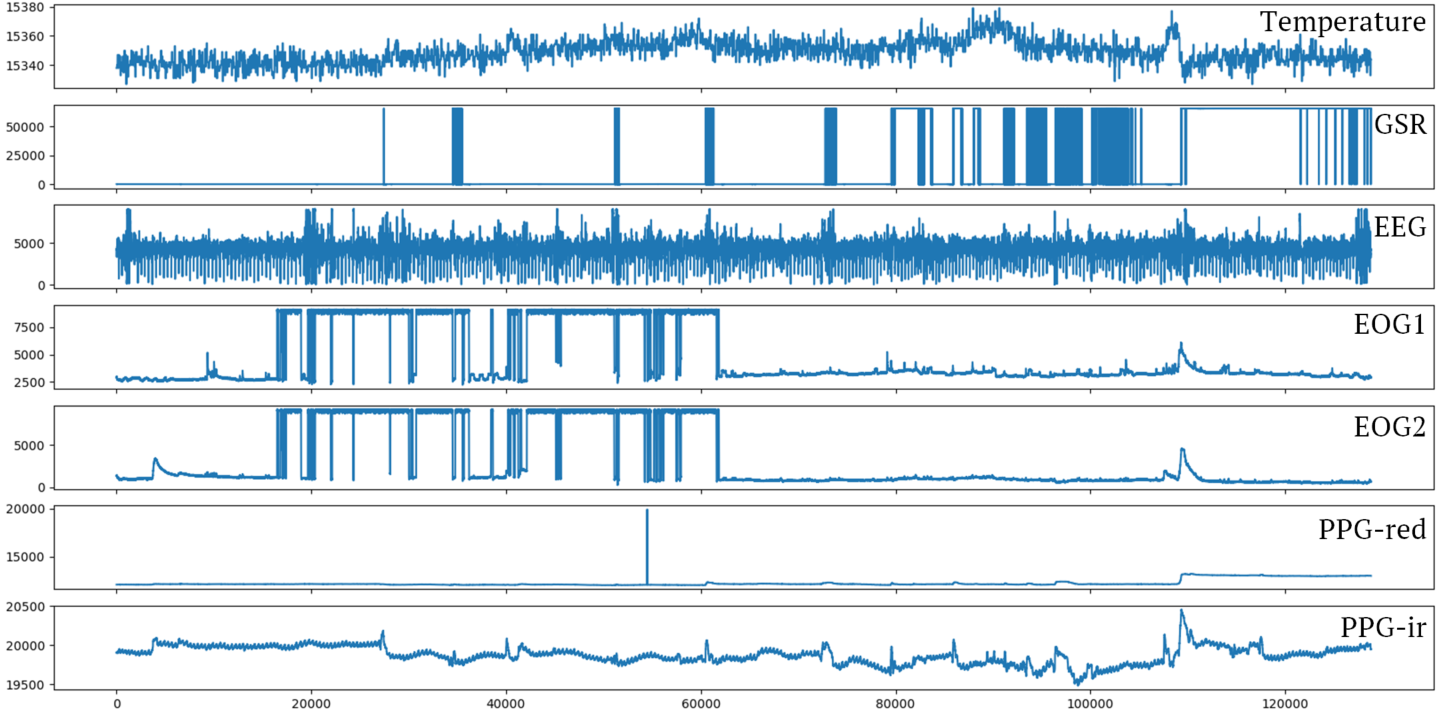
\includegraphics[width=\textwidth]{Images/bad_signals.png} 
\vspace{-0.3cm} \caption[Sensoraufzeichnungen von Daten]{ Sensoraufzeichnungen von Daten, die im Rahmen des ELISE-Projekts von einem der drei getesteten Probanden erfasst wurden. Die x-Achse repr{\"a}sentiert die Zeit und die y-Achse die Sensorwerte. Die in den Daten von GSR und den beiden EOG-Kan{\"a}len sichtbaren Unregelm{\"a}{\ss}igkeiten deuten auf Probleme mit der Hardware hin. }
\label{fig:bad_signals} \end{figure} \vspace{0.5cm}


\begin{figure}[H]
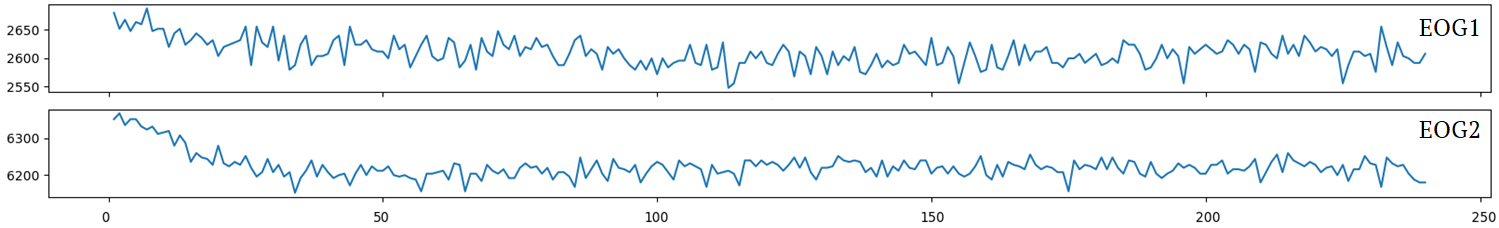
\includegraphics[width=\textwidth]{Images/zoom.png} 
\vspace{-0.3cm} \caption[Nahaufnahme von Rauschen in Daten]{ Nahaufnahme der im Rahmen des ELISE-Projekts erworbenen EOG-Kan{\"a}le von einem der drei getesteten Probanden. Das Vorhandensein von Rauschen in den Daten ist sichtbar, das zu Unregelm{\"a}{\ss}igkeiten in den Signalformen f{\"u}hrt. }
\label{fig:zoom} \end{figure} \vspace{0.5cm}




Der Hauptgrund, warum DNNs keine überzeugenden Ergebnisse lieferten liegt wahrscheinlich an der Erkennungsraten f{\"u}r die am wenigsten vertretenen Klassen (insbesondere ``Frustration'').
Wir gehen davon aus, dass dieses Ph{\"a}nomen durch die relativ geringe Gr{\"o}{\ss}e unseres Datensatzes verursacht wird. 
Ähnlich wie bei den handgefertigten Merkmalen, wird bei den DNNs auch von einem Overfitting an die Probenaden ausgegangen.
Das liegt daran, dass die Performance bei einem Probanden-unabhänigen Datensatz von 47,99\% auf nur 30,91\% sinkt.
Mit einem deutlich größeren Datensatz erwarten wir eine bessere Performance der DNNs.\\






Allgemein deuten die Ergebnisse aber trotzdem darauf hin, dass unser biomedizinisches Datenerfassungssystem zur Emotionserkennung erfolgreich eingesetzt werden k{\"o}nnte, um ein intelligent adaptives Lernsystems zu verbessern. 
Zuk{\"u}nftige Arbeiten werden die Verfeinerung des Multisensor-Datenerfassungsger{\"a}tes, die Erfassung weiterer und gr{\"o}{\ss}erer Datens{\"a}tze f{\"u}r die weitere Mustererkennungsanalyse und die Analyse der Wirksamkeit des Emotionserkennungssystems in einem VR-affektiven Lernkontext beinhalten.